\chapter{Testowanie systemu}

System został przetestowany manualnie poprzez interfejs graficzny oraz poprzez analizę zapytań SQL wykonywanych przez klasę \texttt{ZajeciaDAO}. Testy przeprowadzono w środowisku lokalnym z bazą danych \textbf{PostgreSQL}.

\section{Testy logowania}

Przetestowano poprawność działania formularza logowania:

\begin{figure}[H]
\centering
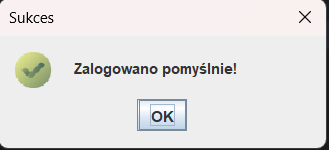
\includegraphics[width=0.4\textwidth]{figures/approve/approve_login.png}
\caption{Logowanie zakończone sukcesem}
\end{figure}

\begin{figure}[H]
\centering
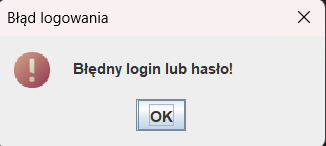
\includegraphics[width=0.4\textwidth]{figures/Errors/bad_login.png}
\caption{Blad logowania – nieprawidlowe dane}
\end{figure}

\section{Testy dodawania zajęć}

Przetestowano dodawanie różnych typów zajęć:

\begin{itemize}
    \item Dodanie zajęć typu \texttt{Projekt} – poprawne wstawienie danych do bazy;
    \item Sprawdzenie walidacji grupy i sali – przy próbie konfliktu system wyświetla stosowny komunikat;
    \item Dodanie zajęć tylko dla jednej grupy (np. \texttt{grupaA}) działa prawidłowo.
\end{itemize}

\begin{figure}[H]
\centering
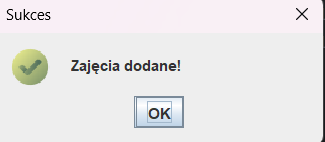
\includegraphics[width=0.5\textwidth]{figures/approve/add_zajecia_succesfull.png}
\caption{Potwierdzenie dodania zajęć}
\end{figure}

\section{Testy filtrowania danych}

Sprawdzono poprawność działania filtrów:

\begin{itemize}
    \item Filtrowanie po dniu i grupie – poprawne ograniczenie wyników;
    \item Filtrowanie po typie zajęć i przedmiocie – wyświetlane są tylko pasujące rekordy;
    \item Filtrowanie nieistniejących danych – system poprawnie wyświetla pustą tabelę bez błędów.
\end{itemize}

\section{Testy edycji i usuwania zajęć}

Przetestowano operacje modyfikacji i usuwania danych:

\begin{itemize}
    \item Edycja sali i prowadzącego – zmiany są natychmiast widoczne w tabeli GUI;
    \item Usunięcie zajęć z bazy powoduje ich zniknięcie z interfejsu;
    \item Obsługa wyjątków SQL przy próbie edycji nieistniejącego rekordu działa prawidłowo.
\end{itemize}

\begin{figure}[H]
\centering
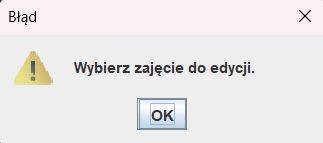
\includegraphics[width=0.5\textwidth]{figures/Warning/select_zajecia_to_edit.png}
\caption{Brak zaznaczonego rekordu do edycji}
\end{figure}

\begin{figure}[H]
\centering
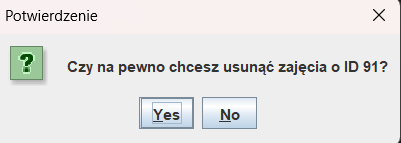
\includegraphics[width=0.5\textwidth]{figures/Warning/delete_warning.png}
\caption{Potwierdzenie usuniecia zajec}
\end{figure}

\begin{figure}[H]
\centering
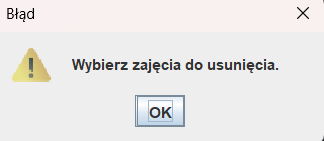
\includegraphics[width=0.5\textwidth]{figures/Warning/select_zajecia.png}
\caption{Brak zaznaczonego rekordu do usuniecia}
\end{figure}

\section{Testy walidacji danych}

Sprawdzono poprawność działania walidacji formularza:

\begin{itemize}
    \item Puste pola – system wyświetla komunikat bledu i nie zapisuje danych;
    \item Nieprawidlowe dane (np. litery w polu godzina) – poprawna obsluga bledu i komunikat;
    \item Proba dodania zajec do juz zajetej sali – system blokuje takie dodanie;
    \item Konflikt grupy – uzytkownik otrzymuje odpowiedni alert.
\end{itemize}

\begin{figure}[H]
\centering
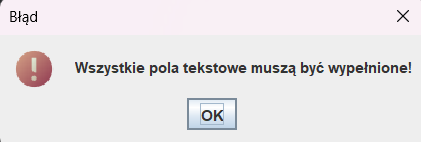
\includegraphics[width=0.55\textwidth]{figures/Errors/add_panel_error.png}
\caption{Puste pola formularza – komunikat bledu}
\end{figure}

\begin{lstlisting}[caption={Walidacja pustych pol}, label={lst:puste}]
if (kierunek.isEmpty() || przedmiot.isEmpty() || prowadzacy.isEmpty()) {
    JOptionPane.showMessageDialog(null, "Wszystkie pola tekstowe musza byc wypelnione!",
        "Blad", JOptionPane.WARNING_MESSAGE, warningIcon);
    return;
}
\end{lstlisting}

\begin{figure}[H]
\centering

\includegraphics[width=0.55\textwidth]{figures/Errors/sala_zajeta_error.png}
\caption{Blad – sala juz zajeta w tym terminie}
\end{figure}

\begin{lstlisting}[caption={Sprawdzanie dostepnosci sali}, label={lst:sala}]
if (dao.czySalaZajeta(sala, dzien, godzina, null)) {
    JOptionPane.showMessageDialog(null, "Sala jest juz zajeta w tym dniu i godzinie!",
        "Konflikt", JOptionPane.WARNING_MESSAGE, warningIcon);
    return;
}
\end{lstlisting}

\begin{lstlisting}[caption={Sprawdzenie konfliktu grupy}, label={lst:grupa}]
JOptionPane.showMessageDialog(null, "Wybrana grupa ma juz zajecia w tym dniu i godzinie!",
    "Konflikt", JOptionPane.WARNING_MESSAGE, warningIcon);
return;
\end{lstlisting}
